\documentclass[10pt,a4paper]{article}
\usepackage[latin3]{inputenc}
\usepackage{amsmath}
\usepackage{amsfonts}
\usepackage{amssymb}
\usepackage{graphicx}
\author{Ricardo Arango - Big Bang Data}
\title{Modelo de Deserci�n en Clientes}
\begin{document}
\maketitle
	\noindent La fuga de clientes se define como el \textit{Movimiento de un cliente de un proveedor de servicio a otro}, mientras que la gesti�n de fuga de clientes describe el proceso por el cual el operador del servicio intenta evitar la fuga del cliente. En consecuencia, la utilizaci�n de modelos predictivos que permitan \textbf{identificar clientes en situaci�n de riesgo de fuga}, permite al operador dirigir esfuerzos en prevenir la salida del cliente.
	\section{Los Datos}
		La variable \textit{target} corresponde a la variable objetivo que se quiere predecir. En este caso, el abandono voluntario de clientes, esta variable es de car�cter booleano, \textbf{FALSE: cliente permanece con sus servicios � TRUE: clientes los abandona voluntariamente}.
		
		
		\begin{figure}[h]
			\centering
			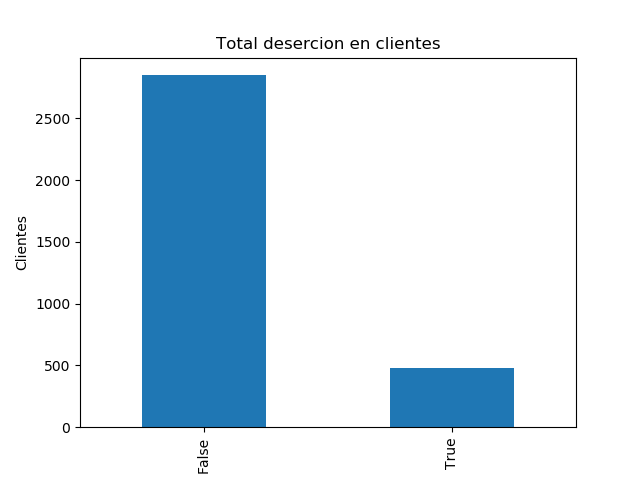
\includegraphics[width=0.5\textwidth]{count_churn}
		\end{figure}
		El $Odd_{desercion}=0.17$, es decir: por cada cliente que abandona los servicios, 6 clientes no lo hacen.
		\begin{equation*}
			Odd_{desercion}\approx\frac{1}{6}
		\end{equation*}
		La  meta es reducir dicho n�mero lo m�ximo posible aumentando, considerablemente, la cantidad de usuarios que permanecen con sus servicios.

		\vspace{1cm}
		A continuaci�n enumeraremos los rasgos m�s caracter�sticos presentes (hist�ricamente) en los  clientes que deciden abandonar los servicios. Esto con el fin de identificar posibles alarmas y evitar la fuga de clientes.
		

		\begin{figure}[h]
			\centering
			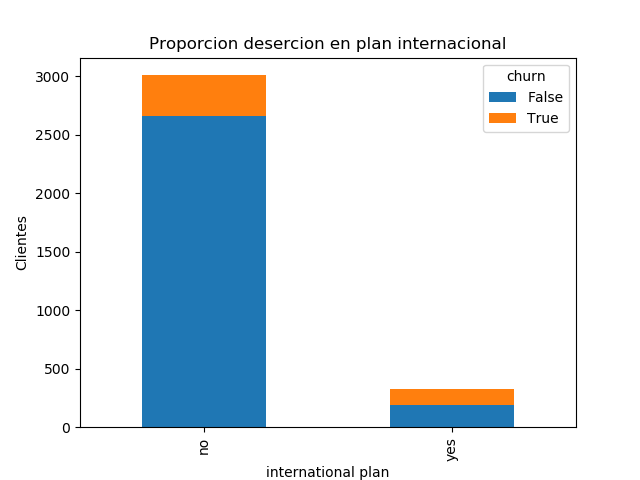
\includegraphics[width=0.5\textwidth]{prop_churn_inrternational}
		\end{figure}
		
		La medida del \textit{ratio} entre las variables de deserci�n y plan internacional es:
		\begin{equation*}
			ratio_{desercion,p-internacional} = 5.67
		\end{equation*}
		De dicho n�mero podemos inferir que la relaci�n entre estas dos variables es fuerte, es decir: \textbf{es muy probable que alguien con un plan internacional deserte}.
		\vspace{0.5cm}
				\begin{figure}[h]
			\centering
			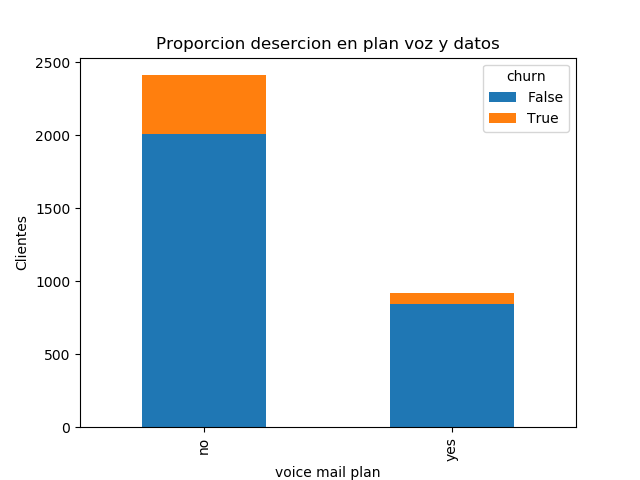
\includegraphics[width=0.5\textwidth]{prop_churn_voice_mail}
		\end{figure}
		
		La medida del \textit{ratio} entre las variables de deserci�n y plan de datos es:
		\begin{equation*}
		ratio_{desercion,p-datos} = 0.47
		\end{equation*}
		De dicho n�mero podemos inferir que la relaci�n entre estas dos variables es fuerte, es decir: \textbf{es muy probable que alguien con un plan de datos no deserte}.
		\vspace{0.5cm}
\end{document}